\documentclass[12pt]{article}

%DEFINIZIONE DEI PACCHETTI GENERICI
\usepackage[a4paper,top=3.5cm,bottom=2.5cm,left=3cm,right=3cm]{geometry}
\usepackage{times}
\usepackage{titlesec}
%\usepackage{lipsum}
\usepackage{titletoc}

%DEFINIZIONE DEI PACCHETTI MATEMATICI
\usepackage{amsmath}
\usepackage{amsfonts}
\usepackage{amssymb}
\usepackage{amsthm}

%DEFINIZIONE DEI PACCHETTI GRAFICI
\usepackage{tikz}
    \usetikzlibrary{graphs}
    \usetikzlibrary{matrix,decorations.pathreplacing}
    \pgfkeys{tikz/mymatrixenv/.style={decoration=brace, 
                                      every left delimiter/.style={xshift=4pt}, 
                                      every right delimiter/.style={xshift=-4pt}}}
    \pgfkeys{tikz/mymatrix/.style={matrix of math nodes, 
                                   inner sep=5pt, 
                                   row sep=0pt, 
                                   column sep=50pt, 
                                   nodes={inner sep=6pt}}}


%STILE DELLE PROPOSIZIONI
\theoremstyle{plain}

% Intestazioni in ingelse
\newtheorem{thm}{Theorem}[section]
\newtheorem{lem}[thm]{Lemma}
\newtheorem{prop}[thm]{Proposition}
\newtheorem{cor}[thm]{Corollary}
\newtheorem{defn}[thm]{Definition}
\newtheorem{rmk}[thm]{Remark}
\newtheorem{ex}[thm]{Example}
\newtheorem{prob}[thm]{Problem}
\newtheorem*{quest*}{Question}
\newtheorem*{notat*}{Notation}

% Intestazioni in italiano
%\newtheorem{thm}{Teorema}[section]
%\newtheorem{lem}[thm]{Lemma}
%\newtheorem{prop}[thm]{Proposizione}
%\newtheorem{cor}[thm]{Corollario}
%\newtheorem{defn}[thm]{Definizione}
%\newtheorem{rmk}[thm]{Osservazione}
%\newtheorem{ex}[thm]{Esempio}
%\newtheorem{prob}[thm]{Problema}
%\newtheorem*{notat*}{Notazione}
%\newtheorem*{quest*}{Domanda}

%STILE DELLE SEZIONI
\titleformat{\section}
{\normalfont \scshape \centering}{\thesection.}{0,5em}{}
%\titlespacing*{\section}{0pt}{50pt}{0.5cm}

\titleformat{\subsection}
{\normalfont \bfseries }{\normalfont \thesubsection.}{0,5em}{}
%\titlespacing*{\subsection}{0pt}{50pt}{0.5cm}

\titlecontents{section}[0cm]{}
{\normalfont \thecontentslabel. \enspace}
{\hspace*{-5.3em}}
{ \hfill \normalfont \contentspage}

\titlecontents{subsection}[0cm]{}
{\normalfont \thecontentslabel. \enspace}
{\hspace*{-5.3em}}
{ \hfill \normalfont \contentspage}

%OPZIONI PER LA BIBLIOGRAFIA
\usepackage[
%backend=bibtex,
backend=biber,
style=alphabetic,
]{biblatex}
\addbibresource{bibliography.bib}
\AtNextBibliography{\small}

% imposto lo stile dell'abstract
\renewcommand{\abstractname}{\normalfont \scshape \centering Abstract}

%INIZIO DEL DOCUMENTO
\begin{document}

    % impostazione del titolo
	\begin{center}
	    \fontsize{12pt}{0pt} % dimensioni del titolo
        \textbf{\MakeUppercase{A basis for the primitive elements by counting symmetric chains}} % titolo
	\end{center}

    %impostazione dell'indice
    {
    \fontsize{12pt}{0pt} % dimensioni delle voci
    \tableofcontents % print della tavola dei contenuti
    }

    %INIZIA A SCRIVERE QUI
    \fontsize{12pt}{0pt} % dimensione del font e spaziatura tra le righe

    \section{Symmetric chain decomposition}

    In this first section we introduce symmetric chain decompositions for a poset. 
    Later on we use this decomposition for divisibility poset of monomials.
    A symmetric chain decomposition of a poset is a way to decompose it in a disjoint union of symmetric total ordered set.

    \begin{defn}
        Let $(\mathcal{P}, \le)$ a ranked poset with rank function $rk : \mathcal{P} \longrightarrow \mathbb{N}$, we say that the elements $x_1, \dots, x_h \in \mathcal{P}$ form a symmetric chain if :
        \begin{enumerate}
            \item $x_{i+1} \gtrdot x_{i}$ for all $i < h$;
            \item $rk(x_1) + rk(x_h) = rk(\mathcal{P}).$
        \end{enumerate}
        where $rk(\mathcal{P})$ is the largest rank in $\mathcal{P}$.
    \end{defn}
    
    \begin{rmk}
        Suppose that $rk(\mathcal{P}) = k$, then consider $x_1, \dots, x_h \in \mathcal{P}$ a symmetric chain in $\mathcal{P}$. Then, by condition (2) of the above definition we have that $rk(x_1) = k - rk(x_h)$, so the length of the chain above the middle rank of the poset $\mathcal{P}$ is equal to the length of the chain under the middle rank of the poset $\mathcal{P}$.
    \end{rmk}
    
    We give here some examples.
    
    \begin{ex} \label{ex:chains}
        \begin{enumerate}
            \item Let $X$ be a finite set, consider the power set $\mathcal{P}(X)$ with rank function $rk : \mathcal{P}(X) \longrightarrow \mathbb{N}$ defined by $rk(A) = |A|$. Then a collection $A_1, \dots, A_h \in \mathcal{P}(X)$ form a symmetric chain if:
            \begin{enumerate}
                \item $A_i \subset A_{i+1}$ and $|A_{i+1}| = 1 + |A_i|$ for $i<h$;
                \item $|A_1| + |A_h| = |X|$.
            \end{enumerate}
            Consider for example the set $X = \{a,b,c,d\}$, in Figure \ref{fig:symmchain1} is depicted a symmetric chain decomposition of $\mathcal{P}(X)$.
    
            \begin{figure}[h!]
            \begin{center} 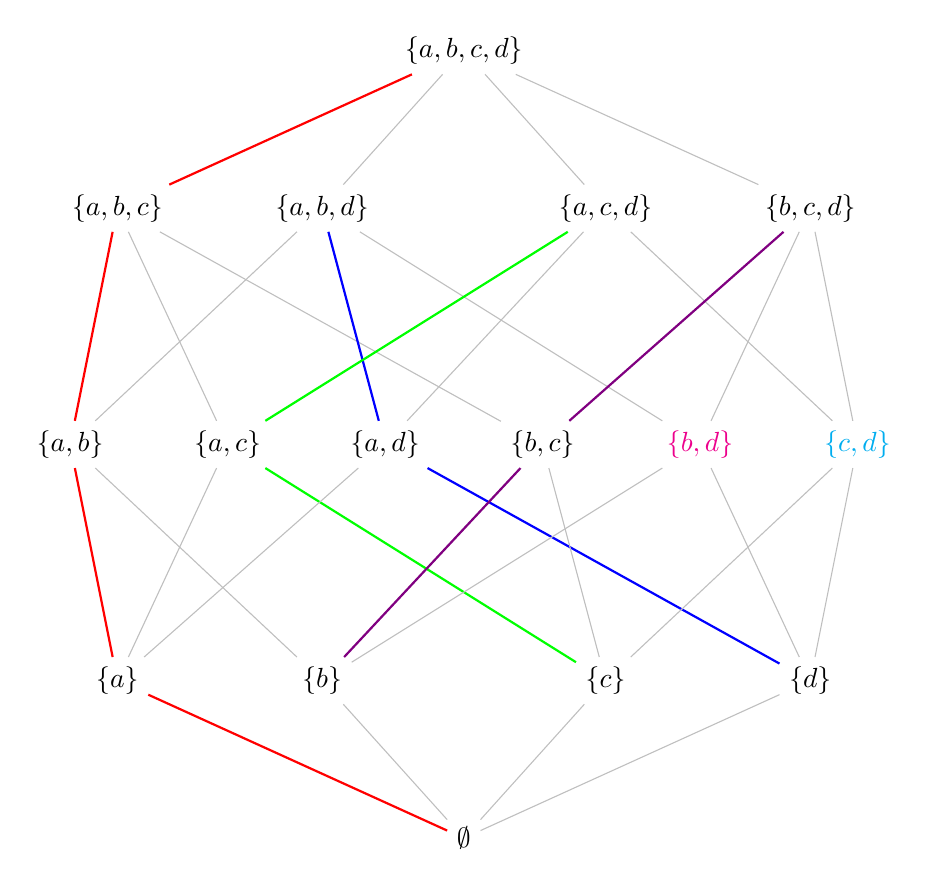
\begin{tikzpicture}
                \node (top) at (0,0) {$\{ a, b, c, d \}$};
                \node (n1) at (-4.4, -2)  {$\{a, b, c \}$};
                \node (n2) at (-1.8, -2)  {$\{a, b, d\}$};
                \node (n3) at (1.8, -2)  {$\{a, c, d \}$};
                \node (n4) at (4.4, -2)  {$\{ b, c, d \}$};
    
                \draw[thick, red] (top) -- (n1);
                \draw[lightgray] (top) -- (n2);
                \draw[lightgray] (top) -- (n3);
                \draw[lightgray] (top) -- (n4);
    
                \node (n5) at (-5, -5)  {$\{ a,b \}$};
                \node (n6) at (-3, -5)  {$\{ a,c \}$};
                \node (n7) at (-1, -5)  {$\{ a,d \}$};
                \node (n8) at (1, -5)  {$\{ b,c \}$};
                \node[magenta] (n9) at (3, -5)  {$\{ b, d \}$};
                \node[cyan] (n10) at (5, -5)  {$\{ c,d \}$};
    
                \draw[thick, red] (n1) -- (n5);
                \draw[lightgray] (n1) -- (n6);
                \draw[lightgray] (n1) -- (n8);
                \draw[lightgray] (n2) -- (n5);
                \draw[thick, blue] (n2) -- (n7);
                \draw[lightgray] (n2) -- (n9);
                \draw[thick, green] (n3) -- (n6);
                \draw[lightgray] (n3) -- (n7);
                \draw[lightgray] (n3) -- (n10);
                \draw[thick, violet] (n4) -- (n8);
                \draw[lightgray] (n4) -- (n9);
                \draw[lightgray] (n4) -- (n10);
                
                
                \node (n11) at (-4.4, -8)  {$\{ a\}$};
                \node (n12) at (-1.8, -8)  {$\{ b \}$};
                \node (n13) at (1.8, -8)  {$\{ c \}$};
                \node (n14) at (4.4, -8)  {$\{ d \}$};
    
                \draw[thick, red] (n5) -- (n11);
                \draw[lightgray] (n5) -- (n12);
                \draw[lightgray] (n6) -- (n11);
                \draw[thick, green] (n6) -- (n13);
                \draw[lightgray] (n7) -- (n11);
                \draw[thick, blue] (n7) -- (n14);
                \draw[thick, violet] (n8) -- (n12);
                \draw[lightgray] (n8) -- (n13);
                \draw[lightgray] (n9) -- (n12);
                \draw[lightgray] (n9) -- (n14);
                \draw[lightgray] (n10) -- (n13);
                \draw[lightgray] (n10) -- (n14);
                
                \node (bottom) at (0, -10) {$\emptyset$};
    
                \draw[thick, red] (bottom) -- (n11);
                \draw[lightgray] (bottom) -- (n12);
                \draw[lightgray] (bottom) -- (n13);
                \draw[lightgray] (bottom) -- (n14);
                
            \end{tikzpicture} \end{center}
            \caption{A symmetric chain decomposition of $\mathcal{P}(\{a,b,c,d\})$}
            \label{fig:symmchain1}
            \end{figure}
            Where the symmetric chains are:
            \[ \emptyset \subset \{a\} \subset \{a,b\} \subset \{a,b,c\} \subset \{a,b,c,d\} \]
            \[ \{b\} \subset \{b,c\} \subset \{b,c,d\}\]
            \[ \{c\} \subset \{a,c\} \subset \{a,c,d\}\]
            \[ \{d\} \subset \{a,d\} \subset \{a,b,d\}\]
            \[ \{b,d\} \]
            \[ \{ c,d \}. \]
        
            \item Consider $n \in \mathbb{N}$ and the poset ordered by divisibility $(Div(n), \mid\,)$ with rank function $rk(d) = $"number of prime factor of $d$ counted with multiplicity", then $d_1, \dots, d_h \in Div(n)$ form a symmetric chain if:
            \begin{enumerate}
                \item $d_i$ divides $d_{i+1}$, and $\frac{d_{i+1}}{d_i}$ is prime for each $i < h$;
                \item $rk(d_1) + rk(d_h) = r(m)$.
            \end{enumerate}
    
            For example consider the poset of divisors of $n = 180 = 2^2 \cdot 3^2 \cdot 5$, then a symmetric chains decomposition (depicted in Figure \ref{symmchain2}) is:
                \[ 1 \prec 2 \prec 2^2 \prec 2^2 \cdot 3 \prec 2^2 \cdot 3^2 \prec 2^2 \cdot 3^2 \cdot 5\]
                \[ 3 \prec 2 \cdot 3 \prec 2 \cdot 3^2 \prec 2 \cdot 3^2 \cdot 5\]
                \[ 5 \prec 3 \cdot 5 \prec 2 \cdot 3 \cdot 5 \prec 2^2 \cdot 3 \cdot 5\]
                \[ 3^2 \prec 3^2 \cdot 5\]
                \[ 2 \cdot 5 \prec 2^2 \cdot 5\]
            where with the relation $\prec$ we denote the divisibility relation.
                
    
            \begin{figure}[h!]
            \begin{center} 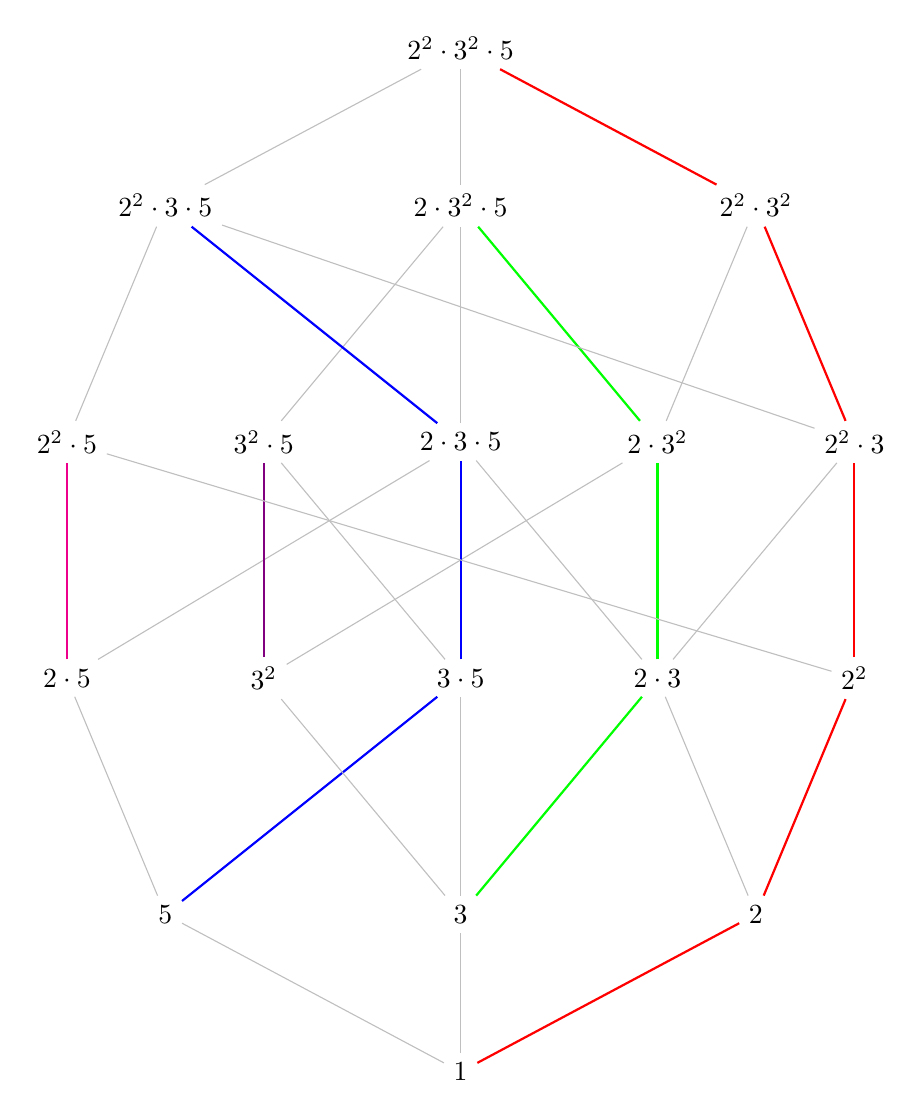
\begin{tikzpicture}
                \node (top) at (0,0) {$2^2 \cdot 3^2 \cdot 5$};
                \node (n1) at (-3.75, -2)  {$2^2 \cdot 3 \cdot 5$};
                \node (n2) at (0, -2)  {$2 \cdot 3^2 \cdot 5$};
                \node (n3) at (3.75, -2)  {$2^2 \cdot 3^2$};
    
                \draw[lightgray] (top) -- (n1);
                \draw[lightgray] (top) -- (n2);
                \draw[thick, red] (top) -- (n3);
    
                \node (n5) at (-5, -5)  {$2^2 \cdot 5$};
                \node (n6) at (-2.5, -5)  {$3^2 \cdot 5$};
                \node (n7) at (0, -5)  {$2\cdot 3\cdot 5$};
                \node (n9) at (2.5, -5)  {$2 \cdot 3^2$};
                \node(n10) at (5, -5)  {$2^2 \cdot 3$};
    
                \draw[lightgray] (n5) -- (n1);
                \draw[lightgray] (n6) -- (n2);
                \draw[thick, blue] (n7) -- (n1);
                \draw[lightgray] (n7) -- (n2);
                \draw[thick, green] (n9) -- (n2);
                \draw[lightgray] (n9) -- (n3);
                \draw[lightgray] (n10) -- (n1);
                \draw[thick, red] (n10) -- (n3);
                
                \node (n11) at (-5, -8)  {$2 \cdot 5$};
                \node (n12) at (-2.5, -8)  {$3^2$};
                \node (n13) at (0, -8)  {$3\cdot 5$};
                \node (n14) at (2.5, -8)  {$2 \cdot 3$};
                \node (n15) at (5, -8)  {$2^2$};
    
    
                \draw[thick, magenta] (n11) -- (n5);
                \draw[lightgray] (n11) -- (n7);
                \draw[thick, violet] (n12) -- (n6);
                \draw[lightgray] (n12) -- (n9);
                \draw[lightgray] (n13) -- (n6);
                \draw[thick, blue] (n13) -- (n7);
                \draw[lightgray] (n14) -- (n7);
                \draw[thick, green] (n14) -- (n9);
                \draw[lightgray] (n14) -- (n10);
                \draw[lightgray] (n15) -- (n5);
                \draw[thick, red] (n15) -- (n10);            
                
                \node (n16) at (-3.75, -11)  {$5$};
                \node (n17) at (0, -11)  {$3$};
                \node (n18) at (3.75, -11)  {$2$};
    
    
                \draw[lightgray] (n16) -- (n11);
                \draw[thick, blue] (n16) -- (n13);
                \draw[lightgray] (n17) -- (n12);
                \draw[lightgray] (n17) -- (n13);
                \draw[thick, green] (n17) -- (n14);
                \draw[lightgray] (n18) -- (n14);
                \draw[thick, red] (n18) -- (n15);
                
                \node (bottom) at (0, -13) {$1$};
                
                \draw[lightgray] (bottom) -- (n16);
                \draw[lightgray] (bottom) -- (n17);
                \draw[thick, red] (bottom) -- (n18);
    
                
                
            \end{tikzpicture} \end{center}        
            \caption{A symmetric chain decomposition of Div$(180)$}
            \label{symmchain2}
            \end{figure}
    
        \end{enumerate}
    \end{ex}
    
    We want now to understand how these symmetric chains are constructed.
    We begin with the case of divisibility poset, and then we generalize to a general poset.
    
    \begin{thm}
        The set of divisors of a number ordered by divisibility can be expressed as a disjoint union of symmetric chains.
    \end{thm}
    
    \begin{proof}
        We denote the divisibility relation with $\prec$, i.e.
        \[ r \prec s \iff r \mid s.\]
        Given $m \in \mathbb{N}$, then we proceed by induction on the number of distinct prime number in the decomposition of $m$, $n$.
        \begin{enumerate}
            \item[Case n=1.]  In this case $m = p^{\alpha}$, with $\alpha \in \mathbb{N}$, so we have a symmetric chain:
            \[ 1 \prec p \prec p^2 \prec \dots \prec p^{\alpha -1} \prec p^{\alpha}\]
            containing all the divisors of $m$.
    
            \item[Inductive step.] Suppose that the statement is true for $n$, so for $m = p_1^{k_1} \cdots p_n^{k_n}$.
    
            \item[Case n+1.]     We want to prove that the statement is true for $n+1$. Consider $p$ one prime in the decomposition of $m$, then we can write $m = m_1 \cdot p^{\alpha}$ with $p \not \mid m_1$, then the number of prime number appearing in the decomposition of $m_1$ is $n$.
            By inductive hypothesis we know that the divisibility poset of $m_1$ can be expressed as a disjoint union of symmetric chain, we want to construct symmetric chains for $m$ using the symmetric chains of $m_1$.
            
            Let $d_1, \dots, d_h$ be one of the symmetric chains for $m_1$. Consider now all the divisors of $m$ of the form:
            \[ d_i \cdot p^{\beta}, \, 0 \le \beta \le \alpha, \, 1 \le i \le h.\]
        
            Write all these divisors in a rectangular array and then peel off chains as in the figure:
        
            \begin{center} $\begin{matrix}
                d_1 & d_2 & \dots & d_{h-2} & d_{h-1} & d_{h} \\
                \vspace{3pt}\\
                d_1 p & d_2 p & \dots & d_{h-2} p & d_{h-1}p  &  d_{h}p \\
                \vspace{3pt}\\
                d_1 p^2 & d_2 p^2 & \dots & d_{h-2} p^2 & d_{h-1}p^2  &  d_{h}p^2 \\
                \vspace{3pt}\\
                \vdots & \vdots & \cdots & \vdots & \vdots & \vdots \\
                \vspace{3pt}\\
                d_1 p^{\alpha} & d_2 p^{\alpha} & \dots & d_{h-2} p^{\alpha} & d_{h-1}p^{\alpha}  &  d_{h}p^{\alpha} \\
            \end{matrix}$ \end{center}
            Then the outer layer gives the first chain
            \[d_1 \prec d_2 \prec \dots \prec d_{h-2} \prec d_{h-1} \prec d_{h} \prec d_{h}p \prec \dots \prec d_{h}p^{\alpha} \]
        
            which satisfies condition (1) of the definition of symmetric chain and is symmetric since
            \[ rk(d_1) + rk(d_h p^{\alpha}) = rk(d_1) + rk(d_h) + \alpha = rk(m_1) + rk(p^{\alpha}) = rk(m),\]
            where $rk(d_1) + rk(d_h) = rk(m_1)$ by inductive hypothesis.
            Thus every layer gives a symmetric chain, and every divisor of $m$ can be obtained in this way from a symmetric chain of $m_1$.
        \end{enumerate}
    \end{proof}

    We give here an example to illustrate the procedure given by the theorem.
    \begin{ex}
            In the Example \ref{ex:chains}.2 we can use the theorem to construct in a recursive way the symmetric chain decomposition.
            Consider $m_1 = 2^2$, then we have only a symmetric chains:
            \[ 1 \prec 2 \prec 2^2\]
            now we consider the divisors of type $2^r \cdot 3^k$ with $r,k=0,1,2$ and we obtain the matrix:
            \begin{center} $\begin{matrix}
                1 & 2 & 2^2 \\
                \vspace{3pt}\\
                3 & 2 \cdot 3 & 2^2 \cdot 3 \\
                \vspace{3pt}\\
                3^2 & 2 \cdot 3^2 & 2^2 \cdot 3^2
            \end{matrix}$ \end{center}
            and we obtain three symmetric chains for $2^2 \cdot 3^2$:
            \[ 1 \prec 2 \prec 2^2 \prec 2^2 \cdot 3 \prec 2^2 \cdot 3^2\]
            \[ 3 \prec 2 \cdot 3 \prec 2 \cdot 3^2\]
            \[ 3^2 \]
            Consider the first symmetric chain $1 \prec 2 \prec 2^2 \prec 2^2 \cdot 3 \prec 2^2 \cdot 3^2$, then construct the matrix:
            \begin{center} $\begin{matrix}
                1 & 2 & 2^2 & 2^2 \cdot 3 & 2^2 \cdot 3^2 \\
                5 & 2 \cdot 5 & 2^2 \cdot 5 & 2^2 \cdot 3 \cdot 5 & 2^2 \cdot 3^2 \cdot 5
            \end{matrix}$ \end{center}
            and we obtain two more chains:
            \[ 1 \prec 2 \prec 2^2 \prec 2^2 \cdot 3 \prec 2^2 \cdot 3^2 \prec 2^2 \cdot 3^2 \cdot 5\]
            \[ 5 \prec 2 \cdot 5 \prec 2^2 \cdot 5 \prec 2^2 \cdot 3 \cdot 5.\]
            Doing the same with the chain $3 \prec 2 \cdot 3 \prec 2 \cdot 3^2$:
            \begin{center} $\begin{matrix}
                3 & 2 \cdot 3 & 2 \cdot 3^2 \\
                3 \cdot 5 & 2 \cdot 3 \cdot 5 & 2 \cdot 3^2 \cdot 5
            \end{matrix}$ \end{center}
    
            and obtain two more symmetric chains:
            \[3 \prec 2 \cdot 3 \prec 2 \cdot 3^2 \prec 2 \cdot 3^2 \cdot 5\]
            \[3 \cdot 5 \prec 2 \cdot 3 \cdot 5 \]
    
            Finally consider the one element chain $3^2$:
            \begin{center} $\begin{matrix}
                3^2 \\
                3^2 \cdot 5
            \end{matrix}$ \end{center}
            and obtain the last symmetric chain:
            \[ 3^2 \prec 3^2 \cdot 5.\]
            
            So in the end we found the chains:
            \[ 1 \prec 2 \prec 2^2 \prec 2^2 \cdot 3 \prec 2^2 \cdot 3^2 \prec 2^2 \cdot 3^2 \cdot 5\]
            \[3 \prec 2 \cdot 3 \prec 2 \cdot 3^2 \prec 2 \cdot 3^2 \cdot 5\]
            \[5 \prec 2 \cdot 5 \prec 2^2 \cdot 5 \prec 2^2 \cdot 3 \cdot 5\]        
            \[3 \cdot 5 \prec 2 \cdot 3 \cdot 5 \]
            \[ 3^2 \prec 3^2 \cdot 5.\]
    
            In this case we found a different symmetric chain decomposition respect to the one considered in Example \ref{ex:chains}.2, depicted in Figure \ref{symmchain3}.
    
            \begin{figure}
            \begin{center} 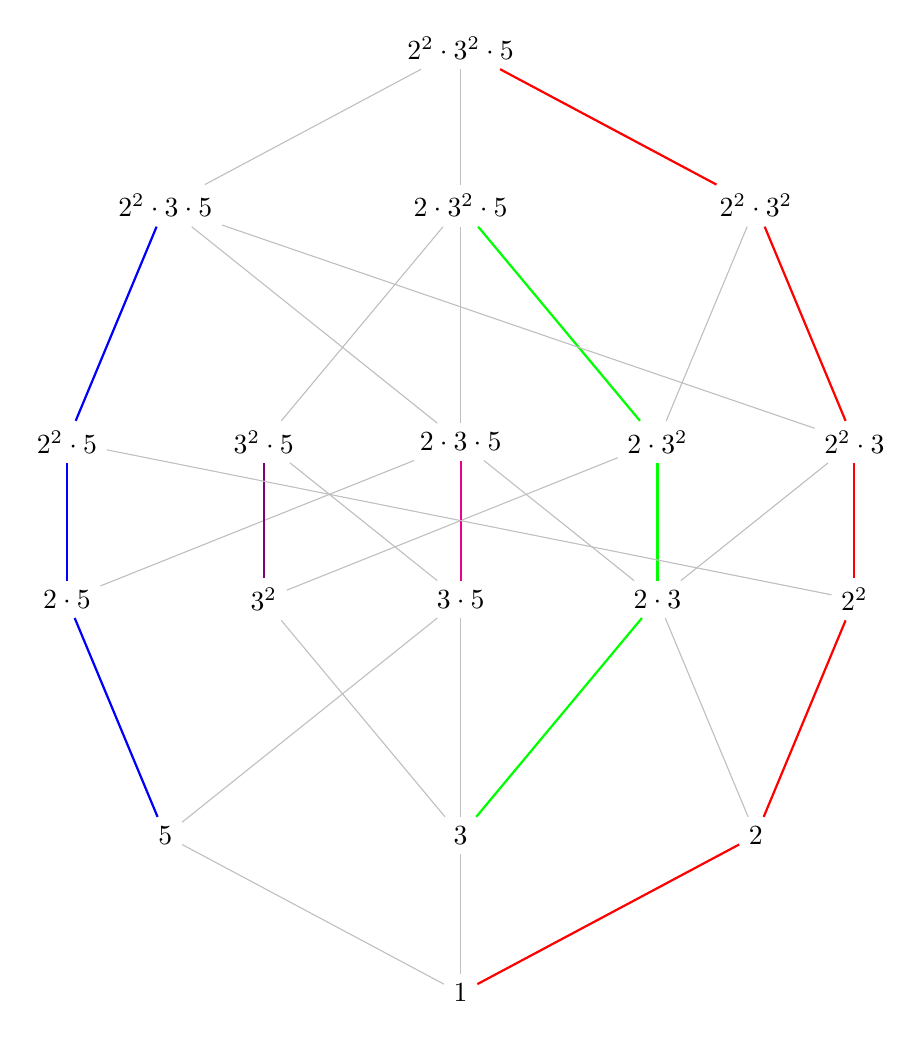
\begin{tikzpicture}
                \node (top) at (0,0) {$2^2 \cdot 3^2 \cdot 5$};
                
                \node (n1) at (-3.75, -2)  {$2^2 \cdot 3 \cdot 5$};
                \node (n2) at (0, -2)  {$2 \cdot 3^2 \cdot 5$};
                \node (n3) at (3.75, -2)  {$2^2 \cdot 3^2$};
    
                \draw[lightgray] (top) -- (n1);
                \draw[lightgray] (top) -- (n2);
                \draw[thick, red] (top) -- (n3);
    
                \node (n5) at (-5, -5)  {$2^2 \cdot 5$};
                \node (n6) at (-2.5, -5)  {$3^2 \cdot 5$};
                \node (n7) at (0, -5)  {$2\cdot 3\cdot 5$};
                \node (n9) at (2.5, -5)  {$2 \cdot 3^2$};
                \node(n10) at (5, -5)  {$2^2 \cdot 3$};
    
                \draw[thick, blue] (n5) -- (n1);
                \draw[lightgray] (n6) -- (n2);
                \draw[lightgray] (n7) -- (n1);
                \draw[lightgray] (n7) -- (n2);
                \draw[thick, green] (n9) -- (n2);
                \draw[lightgray] (n9) -- (n3);
                \draw[lightgray] (n10) -- (n1);
                \draw[thick, red] (n10) -- (n3);
                
                \node (n11) at (-5, -7)  {$2 \cdot 5$};
                \node (n12) at (-2.5, -7)  {$3^2$};
                \node (n13) at (0, -7)  {$3\cdot 5$};
                \node (n14) at (2.5, -7)  {$2 \cdot 3$};
                \node (n15) at (5, -7)  {$2^2$};
    
                \draw[thick, blue] (n11) -- (n5);
                \draw[lightgray] (n11) -- (n7);
                \draw[thick, violet] (n12) -- (n6);
                \draw[lightgray] (n12) -- (n9);
                \draw[lightgray] (n13) -- (n6);
                \draw[thick, magenta] (n13) -- (n7);
                \draw[lightgray] (n14) -- (n7);
                \draw[thick, green] (n14) -- (n9);
                \draw[lightgray] (n14) -- (n10);
                \draw[lightgray] (n15) -- (n5);
                \draw[thick, red] (n15) -- (n10);            
                
                \node (n16) at (-3.75, -10)  {$5$};
                \node (n17) at (0, -10)  {$3$};
                \node (n18) at (3.75, -10)  {$2$};
    
    
                \draw[thick, blue] (n16) -- (n11);
                \draw[lightgray] (n16) -- (n13);
                \draw[lightgray] (n17) -- (n12);
                \draw[lightgray] (n17) -- (n13);
                \draw[thick, green] (n17) -- (n14);
                \draw[lightgray] (n18) -- (n14);
                \draw[thick, red] (n18) -- (n15);
                
                \node (bottom) at (0, -12) {$1$};
                
                \draw[lightgray] (bottom) -- (n16);
                \draw[lightgray] (bottom) -- (n17);
                \draw[thick, red] (bottom) -- (n18);
            \end{tikzpicture} \end{center} 
            \caption{A symmetric chain decomposition for Div$(180)$.}
            \label{symmchain3}
            \end{figure}
    \end{ex}

    \begin{rmk}
        \begin{enumerate}
            \item As seen in the previous two examples symmetric chain decomposition are not unique.
            
            \item The recursive procedure can be extended to monomial. Indeed, consider the monomial $p = x_1 ^{n_1} \cdots x_k ^{n_k}$, then we can consider $x_1, \dots, x_k$ as the prime factors appearing in the decomposition of $p$. So considering the poset of divisors of $p$ ordered by divisibility, we can use the procedure described in the theorem to find a symmetric chain decomposition.
        
            \item The procedure can also be extended to set. It is possible in fact to give a bijective relation between sets and monomial:
            \[ \{1, 2, \dots, n\} \longleftrightarrow x_1 \cdot x_2 \cdots x_n,\]
            and observe that the two relations are equivalent:
            \[ \{i_1, \dots, i_k\} \subseteq \{j_1, \dots, j_r\} \iff x_{i_1} \cdots x_{i_k} \mid x_{j_1} \cdots x_{j_r}.\]
            So we can treat the case of poset and monomial in the same way.
        \end{enumerate}
    \end{rmk}

    \subsection{Application to fibers of nested sets}

        In this section we define a support function on the Feichtner-Yuzvinsky monomial basis and we apply the symmetric chain decomposition to its fibers. 
        
        We recall here the definition of the Feichtner-Yuzvinsky monomial basis for the Chow ring $\mathcal{A}(\mathcal{L}, \mathcal{G})$:
        \[ FY := \left\{ x_{F_1}^{m_1} \cdots x_{F_l}^{m_l} \, : \, N=\{F_1, \dots, F_l \} \in \mathcal{N}(\mathcal{L},\mathcal{G}), \, 1 \le m_i \le m_N(F_i), \, i \in \{ 1, \dots, l\} \right\}\]
        where $m_N(F) = rk(F) - rk(\vee N_{\le F}).$

        Define the function
        \[ supp_+ : FY \longrightarrow \mathcal{N}(\mathcal{L}, \mathcal{G})\]
        called extended support map, as follows
        
            \begin{defn}
                If $m_i \ge 1$ for $1 \le i \le l$, then
                \[ supp_+(x_{F_1}^{m_1} \cdots x_{F_l}^{m_l}) := \{F_1, \dots, F_l \} \cup \{E\}.\]
            \end{defn}    
        \noindent
        Observe that $supp_+$ is well-defined because $\mathcal{N}(\mathcal{L}, \mathcal{G})$ is a simplicial complex, i.e.
        \[ \{F_1, \dots, F_l\} \in \mathcal{N}(\mathcal{L}, \mathcal{G}) \implies \{F_1, \dots, F_l\} \cup \{E \} \in \mathcal{N}(\mathcal{L}, \mathcal{G}). \]

        We use the function $supp_+$ to cover the set $FY$ using its fiber. Consider $N^+ =\{F_1, \dots, F_l, E\} \subset \mathcal{G}$ a $\mathcal{G}$-nested set in the image of $supp_+$ then the fiber has the following description:
        \[ supp_+^{-1} (N^+) = \{x_{F_1}^{m_1} \cdots x_{F_l}^{m_l} \cdot x_E^{m_{l+1}}  \}\]
        where the exponents satisfy the inequalities:
        \[ 1 \le m_i \le m_{N^+}(F_i) - 1, \text{ for } 1 \le i \le l;\]
        \[ 0 \le m_{l+1} \le m_{N^+}(E)- 1.\]

        Consider a nested set $N = \{ F_1, \dots, F_k\}$, and suppose that $N^+ \in Im(supp_+)$, we want to apply the recursive method discussed previously to obtain a symmetric chain decomposition of $supp_+^{-1}(N^+)$.

        To obtain a symmetric chain decomposition we proceed recursively. Observe that since all the elements of the fibers must contain $x_{F_1}, x_{F_2}, \dots, x_{F_k}$ the minimum monomial is $x_{F_1} x_{F_2} \cdots x_{F_k}$.

        Consider the monomial $m = x_1 x_2 \cdots x_k$, we define $Div(m)$ as the divisibility poset where the minimum element is $x_1 x_2 \cdots x_k$, instead of the single variables $x_1, \dots, x_k$.

        \begin{enumerate}
            \item[Case $x_{F_1}$:] Consider the element $m_1  =x_{F_1}^{m_{N^+}(F_1) -1}$,       then the symmetric chain decomposition of $Div(m_1)$ is given by the only chain
                \[ x_{F_1} \prec x_{F_1}^2 \prec x_{F_1}^3 \prec \dots \prec x_{F_1}^{m_{N^+}(F_1)-2} \prec x_{F_1}^{m_{N^+}(F_1)-1}.\]
                \begin{rmk}
                    We omitted $1$ as first element of the chain since we are interested in having all the variables in the minimal polynomial.
                \end{rmk}
            \item[Case $x_{F_1}, x_{F_2}$:]
                To compute the symmetric chain decomposition of $Div(m_2)$, where \[m_2 = x_{F_1}^{m_{N^+}(F1) -1} x_{F_2}^{m_{N^+}(F2) -1},\]
                we consider the symmetric chain decomposition of $Div(m_1)$ and we define a matrix where the $i-th$ row is the chain of $m_1$ multiplied by $x_{F_2}^i$ with $ 1 \le i \le m_{N^+}(F_2) -1$.
                Denoting $m_1 = m_{N^+}(F_1)$ and $m_2 = m_{N^+}(F_2)$, we obtain the matrix

                \begin{center} 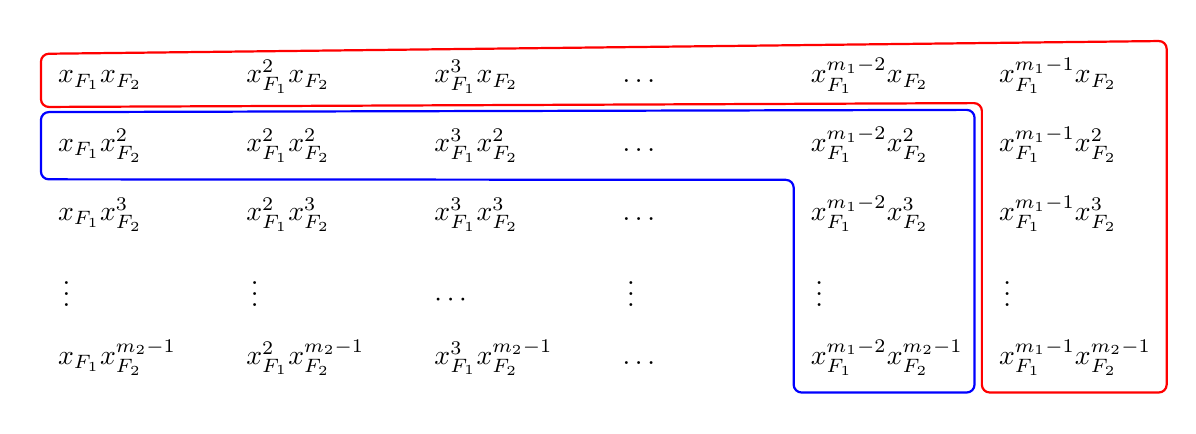
\begin{tikzpicture}[baseline=0cm,mymatrixenv]
                    \matrix [mymatrix,text width=0.6em,align=center] (m) {
                        x_{F_1}x_{F_2} & x_{F_1}^2x_{F_2} & x_{F_1}^3x_{F_2} &\dots & x_{F_1}^{m_1-2} x_{F_2} & x_{F_1}^{m_1-1} x_{F_2} \\
                        x_{F_1}x_{F_2}^2 & x_{F_1}^2x_{F_2}^2 & x_{F_1}^3x_{F_2}^2 &\dots & x_{F_1}^{m_1-2} x_{F_2}^2  & x_{F_1}^{m_1-1} x_{F_2}^2 \\
                        x_{F_1}x_{F_2}^3 & x_{F_1}^2x_{F_2}^3 & x_{F_1}^3x_{F_2}^3 &\dots & x_{F_1}^{m_1-2} x_{F_2}^3 & x_{F_1}^{m_1-1} x_{F_2}^3 \\
                        \vdots & \vdots & \cdots & \vdots & \vdots & \vdots \\
                        x_{F_1}x_{F_2}^{m_2 -1} & x_{F_1}^2x_{F_2}^{m_2 -1} & x_{F_1}^3x_{F_2}^{m_2 -1} &\dots & x_{F_1}^{m_1-2} x_{F_2}^{m_2 -1} & x_{F_1}^{m_1-1} x_{F_2}^{m_2 -1} \\};
                    \pgfmathsetmacro{\offset}{0.5mm}
                        \draw [thick,red,rounded corners=1mm] (m-1-1.north west) -- ([xshift=1.7cm]m-1-6.north east) -- ([xshift=1.7cm]m-5-6.south east) -- (m-5-6.south west) -- ([yshift=0.1cm]m-1-6.south west) -- (m-1-1.south west) -- cycle;
        
                        \draw [thick, blue, rounded corners=1mm] (m-2-1.north west) -- ([xshift=1.65cm]m-2-5.north east) -- ([xshift=1.65cm]m-5-5.south east) -- (m-5-5.south west) -- (m-2-5.south west) -- (m-2-1.south west) -- cycle;
                \end{tikzpicture} \end{center}
                The chains are obtained by the layers of the matrix as depicted in figure.

            \item[Case $x_{F_1},\dots,x_{F_k}$:]    
                Consider now the monomial \[m_k = x_{F_1}^{m_1    -1}x_{F_2}^{m_2 -1} \cdots x_{F_k}^{m_k -1}.\]
                After $k-1$ step, we want to compute the symmetric chain decomposition of $Div(m_k)$.
                To do that, for every chain in the decomposition of $m_{k-1}$ we create a matrix where the $i-th$ row is the selected chain multiplied by $x_{F_k}^i$, with $1 \le i \le m_{N^+}(F_k) -1$. To extract the chains of $Div(m_k)$ we peel off the matrices as before.

            \item[Case $x_{F_1}, \dots, x_E$:]
                The last step is to add $x_E$ to the monomial. Since in the fiber we also have all the monomials without $x_E$, i.e. we consider also the case in which the exponent of $x_E$ is zero, for every chain in $Div(m_k)$ we create a matrix where the $i-th$ row is the selected chain multiplied by $x_E^{i-1}$ where $1 \le i \le m_{N^+}(E)$.
    \end{enumerate}

    INSERIRE UN ESEMPIO.
    
    \subsection{Counting the symmetric chains in the fibers}
    We start by considering the most simple case $N=\{F_1\}$, then $N^+=\{F_1, E\}$.
    
    \begin{prop}
        If $N={F_1}$ then the number of symmetric chains of the decomposition of $supp_+^{-1}(N^+)$ is
        \[ N = \min\{ m_{N^+}(F_1) -1, m_{N^+}(E)\}.\]
    \end{prop}
    
    \begin{proof}
        Call $m_1 = m_{N^+}(F_1)$ and $m_E = m_{N^+}(E)$. Then we have two case
        \begin{enumerate}
            \item[$m_1 > m_E$:]
            in this case we have two possibilities. The first possibility is $m_1 = m_E+1$. In this condition we have that the matrix of chains is a square matrix
            
            \begin{center} \begin{tikzpicture}[baseline=0cm,mymatrixenv]
                    \matrix [mymatrix,text width=0.6em,align=center] (m) {
                        x_{F_1}^{ } & x_{F_1}^2 &\dots & x_{F_1}^{m_1-2}  & x_{F_1}^{m_1-1}\\
                        
                        x_{F_1}^{ }x_{E} & x_{F_1}^2 x_{E} &\dots & x_{F_1}^{m_1-2} x_{E}  & x_{F_1}^{m_1-1} x_{E} \\
                        
                        \vdots & \vdots & \cdots & \vdots & \vdots \\
                        
                        x_{F_1}x_{F_2}^{m_2 -1} & x_{F_1}^2x_{F_2}^{m_2 -1} &\dots & x_{F_1}^{m_1-2} x_{F_2}^{m_2 -1} & x_{F_1}^{m_1-1} x_{F_2}^{m_2 -1} \\
                        
                        x_{F_1}x_{F_2}^{m_2 -1} & x_{F_1}^2x_{F_2}^{m_2 -1} &\dots & x_{F_1}^{m_1-2} x_{F_2}^{m_2 -1} & x_{F_1}^{m_1-1} x_{F_2}^{m_2 -1} \\};
                    
                    \pgfmathsetmacro{\offset}{0.5mm}
                        \draw [thick,red,rounded corners=1mm] (m-1-1.north west) -- ([xshift=1.7cm]m-1-5.north east) -- ([xshift=1.7cm]m-5-5.south east) -- (m-5-5.south west) -- ([yshift=0.1cm]m-1-5.south west) -- (m-1-1.south west) -- cycle;
        
                        \draw [thick, blue, rounded corners=1mm] (m-2-1.north west) -- ([xshift=1.65cm]m-2-4.north east) -- ([xshift=1.65cm]m-5-4.south east) -- (m-5-4.south west) -- (m-2-4.south west) -- (m-2-1.south west) -- cycle;

                        \draw[thick, purple, rounded corners=1mm] (m-4-1.north west) -- ([xshift=1.7cm]m-4-2.north east) -- ([xshift=1.7cm]m-5-2.south east) -- (m-5-2.south west) -- ([yshift=0.5mm]m-4-2.south west) -- ([yshift=0.5mm]m-4-1.south west) -- cycle;

                        \draw [thick, green, rounded corners=1mm] ([yshift=-0.5mm]m-5-1.north west) -- ([xshift=1.65cm]m-5-1.north east) -- ([xshift=1.65cm]m-5-1.south east) -- ([yshift=-0.5mm]m-5-1.south west) -- cycle;
                \end{tikzpicture} \end{center}
                In this case the last chain is formed by on element. Therefore the number of chains is equal to the number of row or column of the matrix which is $m_{N^+}(F_1) -1$.

                The second possibility is when $m_1 > m_E+1$. Here the last chain is horizontal.

                \begin{center} \begin{tikzpicture}[baseline=0cm,mymatrixenv]
                    \matrix [mymatrix,text width=0.6em,align=center] (m) { 
                        x_{F_1}^{ } &  \cdots &x_{F_1}^{m_1 - m_E}  &\dots  & x_{F_1}^{m_1-1}\\
                        
                        \vdots &  & \vdots &  & \vdots \\
                        
                        x_{F_1}x_{E}^{m_E -2}  & \cdots & x_{F_1}^{m_1 - m_E} x_{E}^{m_E -2} & \dots & x_{F_1}^{m_1-1} x_{E}^{m_E -2} \\
                        
                        x_{F_1}x_{E}^{m_E -1} & \cdots & x_{F_1}^{m_1 - m_E}x_{E}^{m_E -1} &\dots & x_{F_1}^{m_1-1} x_{E}^{m_E -1} \\};
                    
                    \pgfmathsetmacro{\offset}{0.5mm}
                        \draw [thick,red,rounded corners=1mm] (m-1-1.north west) -- ([xshift=1.7cm]m-1-5.north east) -- ([xshift=1.7cm]m-4-5.south east) -- (m-4-5.south west) -- ([yshift=0.1cm]m-1-5.south west) -- (m-1-1.south west) -- cycle;

                        \draw [thick, green, rounded corners=1mm] ([yshift=-0.5mm]m-4-1.north west) -- ([xshift=2cm]m-4-3.north east) -- ([xshift=2cm]m-4-3.south east) -- ([yshift=-0.5mm]m-4-1.south west) -- cycle;
                \end{tikzpicture} \end{center}
                Therefore, the number of chains is equal to the number of row which is equal to $m_{N^+}(E)$.

                \item[$m_1 \leq m_E$]
                In this case the last chain is vertical.
                \begin{center} \begin{tikzpicture}[baseline=0cm,mymatrixenv]
                    \matrix [mymatrix,text width=0.6em,align=center] (m) {
                        x_{F_1}^{ } & x_{F_1}^2 & x_{F_1}^3 &\dots  & x_{F_1}^{m_1-1}\\
                        
                        \vdots & \vdots & \vdots & & \vdots \\

                        x_{F_1}x_{E}^{m_1 -2} & x_{F_1}^2x_{E}^{m_1 -2} & x_{F_1}^3 x_{E}^{m_1 -2} &\dots & x_{F_1}^{m_1-1} x_{E}^{m_1 -2} \\
                        
                        \vdots & \vdots & \vdots & & \vdots \\
                        
                        x_{F_1}x_{E}^{m_E -1} & x_{F_1}^2x_{E}^{m_E -1} & x_{F_1}^3 x_{E}^{m_E -1} &\dots &  x_{F_1}^{m_1-1} x_{E}^{m_E -1} \\};
                    
                    \pgfmathsetmacro{\offset}{0.5mm}
                        \draw [thick,red,rounded corners=1mm] (m-1-1.north west) -- ([xshift=1.7cm]m-1-5.north east) -- ([xshift=1.7cm]m-5-5.south east) -- (m-5-5.south west) -- ([yshift=0.1cm]m-1-5.south west) -- (m-1-1.south west) -- cycle;
                        
                        \draw [thick, green, rounded corners=1mm] ([yshift=-0.5mm]m-3-1.north west) -- ([xshift=1.65cm]m-3-1.north east) -- ([xshift=1.65cm]m-5-1.south east) -- ([yshift=-0.5mm]m-5-1.south west) -- cycle;
                \end{tikzpicture} \end{center}

                And the number of chains is equal to the number of column of the matrix, which is equal to $m_{N^+}(F_1)-1$.
        \end{enumerate}

        So, defined $N = $number of chains in the decomposition we have that:
        \[ N = \min\{m_{N^+}(F_1) -1, m_{N^+}(E)\}.\]
    \end{proof}

    \begin{rmk}
        Observe that if we consider the set $\{F_1, F_2 \}$, and we compute the chains in the decomposition of $Div(x_{F_1}^{m_1-1} x_{F_2}^{m_2-1})$ the result is different since we consider the exponent of $x_{F_2}$ to be at least $1$. In this case the result is
        \[ N = \min\{m_{N^+}(F_1), m_{N^+}(F_2)\} -1.\]
    \end{rmk}

    We can also compute the length of this chains, infact
    \begin{prop}
        If $N=\{F_1\}$ then the length of symmetric chains of the decomposition of $supp_+^{-1}(N^+)$ is
        \[ L(\gamma_1) = (m_1 - 1) + (m_E -1) \]
        \[ L(\gamma_i) = L(\gamma_1) - 2(i-1).\]
    \end{prop}

    \begin{proof}
        Call $m_1 = m_{N^+}(F_1)$ and $m_E = m_{N^+}(E)$.
        Calling the chains 
        \begin{center} \begin{tikzpicture}[baseline=0cm,mymatrixenv]
                    \matrix [mymatrix,text width=0.6em,align=center] (m) {
                        \gamma_1: & x_{F_1}^{ } & x_{F_1}^2 &\dots & x_{F_1}^{m_1-2}  & x_{F_1}^{m_1-1}\\
                        
                        \gamma_2: & x_{F_1}^{ }x_{E} & x_{F_1}^2 x_{E} &\dots & x_{F_1}^{m_1-2} x_{E}  & x_{F_1}^{m_1-1} x_{E} \\
                        
                        \vdots & \vdots & \vdots & & \vdots & \vdots \\
                        
                        \gamma_{m_E-2}:& x_{F_1}x_{F_2}^{m_2 -1} & x_{F_1}^2x_{F_2}^{m_2 -1} &\dots & x_{F_1}^{m_1-2} x_{F_2}^{m_2 -1} & x_{F_1}^{m_1-1} x_{F_2}^{m_2 -1} \\
                        
                        \gamma_{m_E-1}: & x_{F_1}x_{F_2}^{m_2 -1} & x_{F_1}^2x_{F_2}^{m_2 -1} &\dots & x_{F_1}^{m_1-2} x_{F_2}^{m_2 -1} & x_{F_1}^{m_1-1} x_{F_2}^{m_2 -1} \\};
                    
                    \pgfmathsetmacro{\offset}{0.5mm}
                        \draw [thick,red,rounded corners=1mm] (m-1-2.north west) -- ([xshift=1.7cm]m-1-6.north east) -- ([xshift=1.7cm]m-5-6.south east) -- (m-5-6.south west) -- ([yshift=0.1cm]m-1-6.south west) -- (m-1-2.south west) -- cycle;
        
                        \draw [thick, blue, rounded corners=1mm] (m-2-2.north west) -- ([xshift=1.65cm]m-2-5.north east) -- ([xshift=1.65cm]m-5-5.south east) -- (m-5-5.south west) -- (m-2-5.south west) -- (m-2-2.south west) -- cycle;

                        \draw[thick, purple, rounded corners=1mm] (m-4-2.north west) -- ([xshift=1.7cm]m-4-3.north east) -- ([xshift=1.7cm]m-5-3.south east) -- (m-5-3.south west) -- ([yshift=0.5mm]m-4-3.south west) -- ([yshift=0.5mm]m-4-2.south west) -- cycle;

                        \draw [thick, green, rounded corners=1mm] ([yshift=-0.5mm]m-5-2.north west) -- ([xshift=1.65cm]m-5-2.north east) -- ([xshift=1.65cm]m-5-2.south east) -- ([yshift=-0.5mm]m-5-2.south west) -- cycle;
                \end{tikzpicture} \end{center}

                The length of $\gamma_1$ is the sum of all his elements. The number of elements in the first line is $m_1 -1$, and in the last row (excluded the first element) is $m_E-1$, therefore:
                \[ L(\gamma_1) = (m_1 - 1) + (m_E -1).\]

                The second chain has $m_1-2$ elements in the row, and $m_E-2$ elements in the column, so
                \[ L(\gamma_2) = (m_1 -2)+ (m_E-2) = m_1 - 1 + m_E -1 - 2 = L(\gamma_1) -2.\]

                Suppose this is true for $n$, so
                \[ L(\gamma_{n}) = L(\gamma_1) - 2(n-1), \]
                then for $n+1$ we have
                \[ L(\gamma_{n+1}) = L(\gamma_n) - 2 = L(\gamma_1) - 2(n-1) - 2 = L(\gamma_1) - 2 n.\]
    \end{proof}

    \begin{rmk}
        In the case we consider $\{F_1, F_2\}$, then the previous result is
        \[ L(\gamma_1) = (m_1 - 1) + (m_2 - 2) \]
        \[ L(\gamma_i) = L(\gamma_1) - 2(i-1).\]
    \end{rmk}

    We now proceed with the case $N = \{ F_1, F_2\}$. In this case $N^+ = \{F_1, F_2, E\}$, and by the privious two proposition we have that the number of chains in the decomposition of $x_1^{m_1 -1} x_{F_2}^{m_2-1}$ is 
    \[ N = \min\{m_{N^+}(F_1), m_{N^+}(F_2)\} - 1.\]
    We call these chains $\gamma_1, \dots, \gamma_N$, their length is given by 
            \[ L(\gamma_1) = (m_1 - 1) + (m_2 - 2) \]
        \[ L(\gamma_i) = L(\gamma_1) - 2(i-1).\]
        
    Now for every $1\le i \le N$, we construct the matrix $M(\gamma_i)$ where 
    \[ M(\gamma_i)(j,k) = \gamma(k)x_E^{j-1}\]
    for $ 1 \le k \le m_1-1$ and $1 \le j \le m_E$.

    We want to compute the number of chains in every $M(\gamma_i)$ and their length.
    We start with $M(\gamma_1)$: the length of the first row is $(m_1 - 1) + (m_2 - 2)$ and the number of row is $m_E$, so as previously in the case $N^+ = \{F_1, E\}$, we have
    \[ N_1 = \min \{ m_1 + m_2 - 3, m_E \}.\]
    The lenght of the second chain is $L(\gamma_1) - 2$, so the number of chain in $M(\gamma_2)$ is 
    \[ N_2 = \min \{ m_1+m_2 - 3 -2, m_E \}, \]
    generalizing
    \[ N_i = \min \{ m_1 + m_2 - 2(i-1) - 1, m_E\}\]
    Calling the chains of $M(\gamma_1)$ $\phi^1_1, \dots, \phi^1_{N_1}$ then we have that
    \[ L(\phi^1_1) = L(\gamma_1) + (m_E-1) = (m_1 - 1) + (m_2 -2) + (m_E -1)\]
    for every other chain we diminish the length by 2, so
    \[ L(\phi^1_i) = L(\gamma_1) - 2(i-1). \]
    Considering the chains $\phi^2_1, \dots, \phi_{N_2}^2$ of $M(\gamma_2)$, we have that
    \[ L(\phi_{1}^2) = L(\gamma_2) + (m_E -1) = L(\gamma_1) - 2 + (m_E -1) = (m_1 -1) + (m_2 -2) - 2 + (m_E -1) = L(\phi_1^1) -2. \]
    Generalizing 
    \[ L(\phi^2_{k}) = L(\phi^2_1) - 2(k-1).\]


    \section{Primitive Elements}

    Given the $FY$ monomial basis, we can cover it with the fibers of the support function. Then we can decompose each fiber in symmetric chains. 
    Now we can define the map $\lambda$ by describing its behavior on the chains of the symmetric chain decomposition of the fibers. Let $a$ be any $FY$-monomial with $k = \deg(a)$, then $a$ lies on a unique fiber $supp_+^{-1}(N^+)$ for some $\mathcal{G}$-nested set $N^+ =\{F_1, \dots ,F_l, E\}$, and on a unique symmetric chain $C_i$, of the symmetric chain decomposition of $supp_+^{-1}(N^+)$,
    \[ C_i = \{ a_\rho \lessdot a_{\rho +1 } \lessdot \dots \lessdot a_{r-\rho-r} \lessdot a_{r-\rho}\},\]
    where $\deg(a_j) = j$ with $j = \rho, \rho +1 , \dots, r- \rho -1, r - \rho$.

    Then, since $a \in C_i$, then exits $k \in \{ \rho, \rho +1 , \dots, r- \rho -1, r - 
    \rho \}$, such that $a = a_k$, so we define:
    \[ \lambda (a) := a_{k+1},  \  k<\frac{r}{2}.\]

    \begin{rmk}
        The map $\lambda$ is an injection
        \[ \lambda : FY^{k} \longrightarrow FY^{k+1},\]
        and it is a deformation of the Lefschetz operator.
    \end{rmk}

    We give here an example.
    \begin{ex} \label{ex:fiber}
    
        Let $\mathcal{L} = \mathcal{L}_{\mathcal{M}}$ be the lattice of flats of a simple matroid $\mathcal{M}$ having $rk(E) = 10 = r+1$ with $r=9$ and $\mathcal{G} = \mathcal{G_{\max}}$. Consider a $\mathcal{G}$-nested set $N^+ = \{F_1, F_2, E\}$ where $F_1 < F_2$ are flats with $rk(F_1) = 3$, $rk(F_2) = 7$. Linearly ordering $\{F_1, F_2 \}$ as $(F_1, F_2)$, then the divisibility poset on the fiber $supp_+^{-1}(\{F_1, F_2, E \})$ is depicted in Figure \ref{fig:suppfiber1}.
        And a possible choice of symmetric chain decomposition looks as depicted in Figure \ref{fig:symmchainsupp}.
        
        \begin{figure}[h!]
        \begin{center} 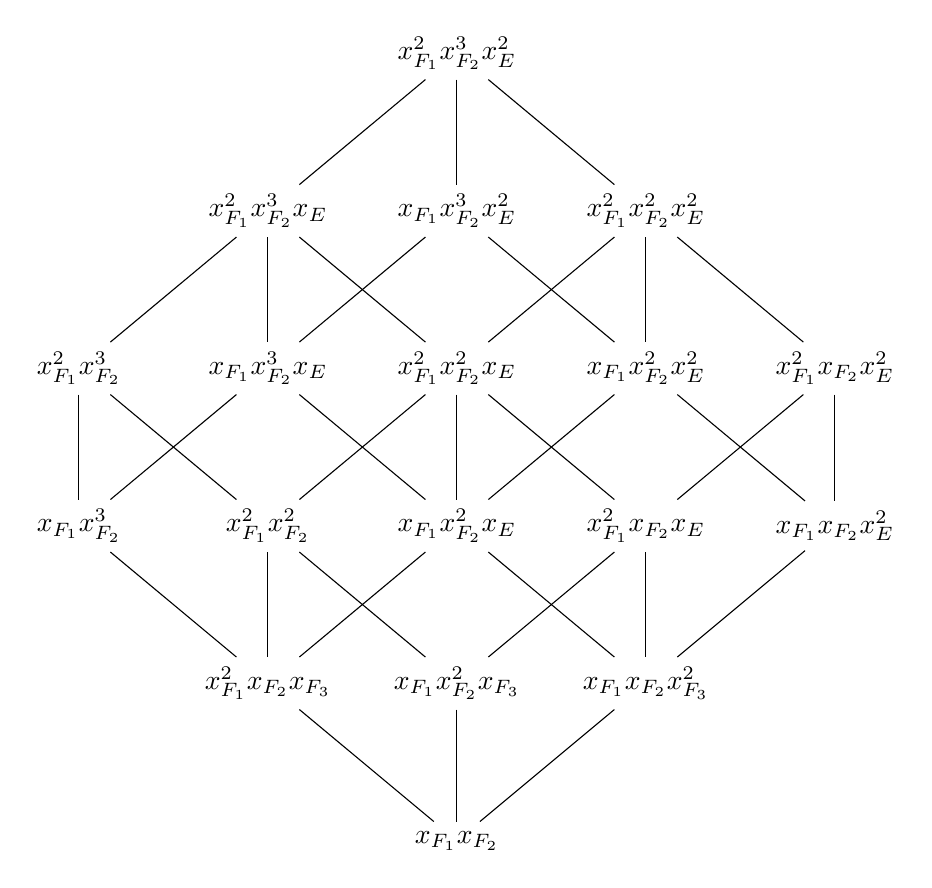
\begin{tikzpicture}
            \node (top) at (0,0) {$x_{F_1}^2x_{F_2}^3x_E^2$};
                    
            \node (n1) at (-2.4, -2)  {$x_{F_1}^2x_{F_2}^3x_E$};
                    \node (n2) at (0, -2)  {$x_{F_1}x_{F_2}^3x_E^2$};
                    \node (n3) at (2.4, -2)  {$x_{F_1}^2x_{F_2}^2x_E^2$};
        
                    \draw (top) -- (n1);
                    \draw (top) -- (n2);
                    \draw (top) -- (n3);
                    
                    \node (n5) at (-4.8, -4)  {$x_{F_1}^2x_{F_2}^3$};
                    \node (n6) at (-2.4, -4)  {$x_{F_1}x_{F_2}^3x_E$};
                    \node (n7) at (0, -4)  {$x_{F_1}^2x_{F_2}^2x_E$};
                    \node (n8) at (2.4, -4)  {$x_{F_1}x_{F_2}^2x_E^2$};
                    \node (n9) at (4.8, -4) {$x_{F_1}^2x_{F_2}x_E^2$};
        
                    \draw (n1) -- (n5);
                    \draw (n1) -- (n6);
                    \draw (n1) -- (n7);
                    \draw (n2) -- (n6);
                    \draw (n2) -- (n8);
                    \draw (n3) -- (n7);
                    \draw (n3) -- (n8);
                    \draw (n3) -- (n9);
                                
                    \node (n10) at (-4.8, -6)  {$x_{F_1}x_{F_2}^3$};
                    \node (n11) at (-2.4, -6)  {$x_{F_1}^2x_{F_2}^2$};
                    \node (n12) at (0, -6)  {$x_{F_1}x_{F_2}^2x_E$};
                    \node (n13) at (2.4, -6)  {$x_{F_1}^2x_{F_2}x_E$};
                    \node (n14) at (4.8, -6) {$x_{F_1}x_{F_2}x_E^2$};
        
                    \draw (n5) -- (n10);
                    \draw (n5) -- (n11);
                    \draw (n6) -- (n10);
                    \draw (n6) -- (n12);
                    \draw (n7) -- (n11);
                    \draw (n7) -- (n12);
                    \draw (n7) -- (n13);
                    \draw (n8) -- (n12);
                    \draw (n8) -- (n14);
                    \draw (n9) -- (n13);
                    \draw (n9) -- (n14);
                    
                    \node (n15) at (-2.4, -8)  {$x_{F_1}^2x_{F_2}x_{F_3}$};
                    \node (n16) at (0, -8)  {$x_{F_1}x_{F_2}^2x_{F_3}$};
                    \node (n17) at (2.4, -8)  {$x_{F_1}x_{F_2}x_{F_3}^2$};
        
                    \draw (n10) -- (n15);
                    \draw (n11) -- (n15);
                    \draw (n12) -- (n15);
                    \draw (n11) -- (n16);
                    \draw (n13) -- (n16);
                    \draw (n12) -- (n17);
                    \draw (n13) -- (n17);
                    \draw (n14) -- (n17);
                    
                    \node (bottom) at (0, -10) {$x_{F_1}x_{F_2}$};
        
                    \draw (n15) -- (bottom);
                    \draw (n16) -- (bottom);
                    \draw (n17) -- (bottom);
        \end{tikzpicture} \end{center}
        \caption{Hasse diagram of the fiber $supp_+^{-1}(F_1, F_2, E)$.}
        \label{fig:suppfiber1}
        \end{figure}
        
        
        \begin{figure}[h!]
        \begin{center} 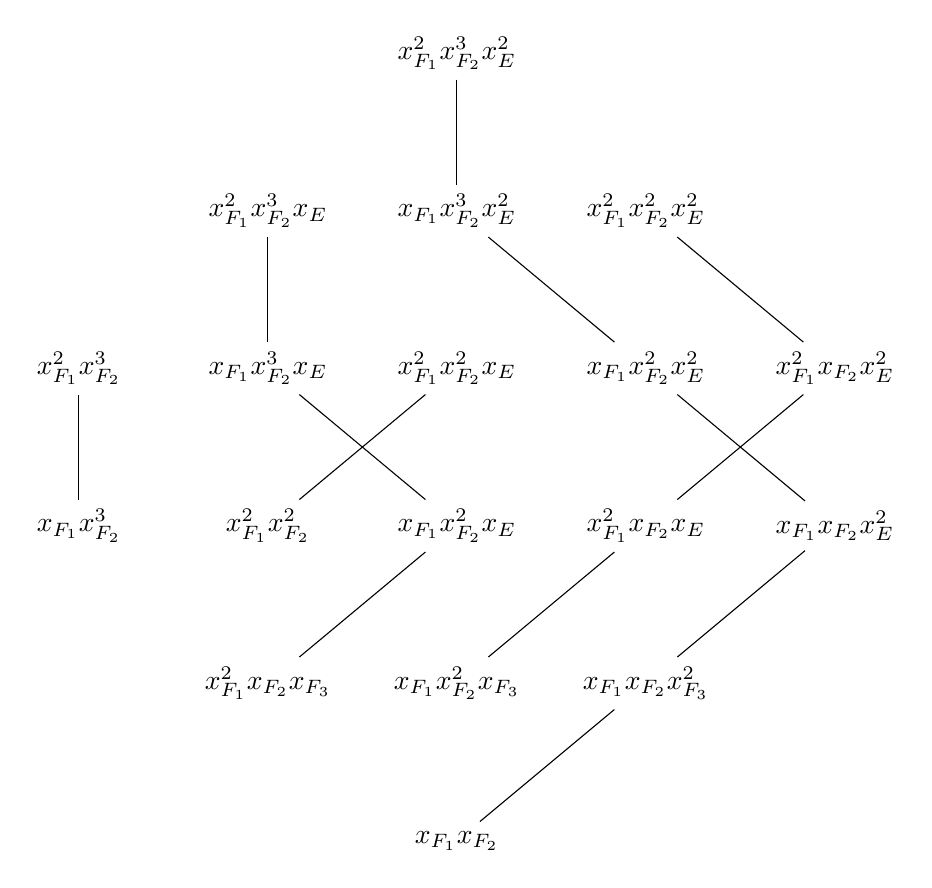
\begin{tikzpicture}
            \node (top) at (0,0) {$x_{F_1}^2x_{F_2}^3x_E^2$};
                    
            \node (n1) at (-2.4, -2)  {$x_{F_1}^2x_{F_2}^3x_E$};
                    \node (n2) at (0, -2)  {$x_{F_1}x_{F_2}^3x_E^2$};
                    \node (n3) at (2.4, -2)  {$x_{F_1}^2x_{F_2}^2x_E^2$};
        
                    \draw (top) -- (n2);
                    
                    \node (n5) at (-4.8, -4)  {$x_{F_1}^2x_{F_2}^3$};
                    \node (n6) at (-2.4, -4)  {$x_{F_1}x_{F_2}^3x_E$};
                    \node (n7) at (0, -4)  {$x_{F_1}^2x_{F_2}^2x_E$};
                    \node (n8) at (2.4, -4)  {$x_{F_1}x_{F_2}^2x_E^2$};
                    \node (n9) at (4.8, -4) {$x_{F_1}^2x_{F_2}x_E^2$};
        
                    \draw (n1) -- (n6);
                    \draw (n2) -- (n8);
                    \draw (n3) -- (n9);
                                
                    \node (n10) at (-4.8, -6)  {$x_{F_1}x_{F_2}^3$};
                    \node (n11) at (-2.4, -6)  {$x_{F_1}^2x_{F_2}^2$};
                    \node (n12) at (0, -6)  {$x_{F_1}x_{F_2}^2x_E$};
                    \node (n13) at (2.4, -6)  {$x_{F_1}^2x_{F_2}x_E$};
                    \node (n14) at (4.8, -6) {$x_{F_1}x_{F_2}x_E^2$};
        
                    \draw (n5) -- (n10);
                    \draw (n6) -- (n12);
                    \draw (n7) -- (n11);
                    \draw (n8) -- (n14);
                    \draw (n9) -- (n13);
                    
                    \node (n15) at (-2.4, -8)  {$x_{F_1}^2x_{F_2}x_{F_3}$};
                    \node (n16) at (0, -8)  {$x_{F_1}x_{F_2}^2x_{F_3}$};
                    \node (n17) at (2.4, -8)  {$x_{F_1}x_{F_2}x_{F_3}^2$};
        
                    \draw (n12) -- (n15);
                    \draw (n13) -- (n16);
                    \draw (n14) -- (n17);
                    
                    \node (bottom) at (0, -10) {$x_{F_1}x_{F_2}$};
        
                    \draw (n17) -- (bottom);
        \end{tikzpicture} \end{center}
        \caption{A possible symmetric chain decomposition for $supp_+^{-1}(F_1, F_2, E)$.}
        \label{fig:symmchainsupp}
        \end{figure}
    \end{ex}    

    Since $\lambda$ send an element of the chain in the next element of the same chain, we can apply it for all the length of the chain and not only for element in $FY^k$ with $k < \frac{r}{2}$. 

    Extend now the map $\lambda$, on a chain $\gamma$, in this way

    \begin{center}
        $\lambda(x_k) = 
        \begin{cases}
             x_{k+1}, \text{ if $x_{k+1} \in \gamma$}\\
            0, \hspace{0.6cm} \text{ if $x_{k+1} \not \in \gamma$ }
        \end{cases}$
    \end{center}

    and we define
    \[ Ker(\lambda) := \{ x \in FY \mid \lambda(x) = 0 \}. \]

    \begin{notat*}
        We denote $\lambda^k = \lambda \circ \lambda \circ \dots \circ \lambda$, for $k$ times. 
    \end{notat*}
    
    \begin{defn}
        Consider $x \in FY^k$, we call $x$ a primitive element if
        \[ x \in P^k:=Ker(\lambda^{r-2k+1} : FY ^k \longrightarrow FY^{r-k+1})\]
    \end{defn}

    \subsection{Characterization of primitive elements}
    Consider a symmetric chain $\gamma$ in $FY$. We depict in figure the action of $\lambda^{r-2k+1}$.
    
    \begin{center} \begin{tikzpicture}[baseline=0cm,mymatrixenv]
        \matrix [mymatrix,text width=0.6em,align=center] (m) {
            \deg & \ & & \deg & \ & \\
            
             &  & \color{blue} \lambda &  &  &  \\
             
            r-k & \bullet & & r-k+1 & \bullet & & \\

            & \mid & & & \mid & \color{blue} \lambda &\\
                        
            r-k-1 & \bullet & & r-k & \bullet & &\\

            & \mid & & &  \mid & &\\
                        
            r-k-2 & \bullet & & r-k-1 & \bullet & &\\

            & \mid & & & \mid & &\\
            
            & \vdots & \color{red}\lambda^{r-2k}  &  & \vdots & \color{red} \lambda^{r-2k}&\\

            & \mid & & & \mid & &\\

            k+2 & \bullet & &  k +1 & \bullet &\\

            & \mid & & & \mid & &\\
            
            k+1 & \bullet & & k & \bullet & &\\

            & \mid & & & \mid & &\\
                        
            k & \bullet & & k-1 & \bullet & &\\};
                    
            \pgfmathsetmacro{\offset}{0.5mm}
                \draw [thick, red, rounded corners=50mm] (m-15-2.east) -- (m-9-3.east) -- (m-3-2.east);
                \draw [thick, blue, rounded corners=15mm] (m-3-2.east) -- ([xshift=-1cm]m-2-3.east) -- (m-1-2.east);

                \draw [thick, red, rounded corners=40mm] (m-13-5.east) -- (m-9-6.east) -- (m-5-5.east);
                \draw [thick, blue, rounded corners=15mm] (m-5-5.east) -- ([xshift=-1cm]m-4-6.east) -- (m-3-5.east);
    \end{tikzpicture} \end{center}

    It's simple to see that the primitive element are the elements that are first in a chain.
    \begin{thm}[Characterization of primitive elements] 
        Let $x \in FY^k$, then        
        \begin{center}$\begin{matrix}
            x \in P^k & \iff & \text{x is the first element of a symmetric chain}.
        \end{matrix}$\end{center}
    \end{thm}

    \begin{proof}
        Let $x \in FY^k$, and suppose $x \in \gamma$ for a certain symmetric chain $\gamma$.
        If $x$ is the first element of $\gamma$, then $\lambda^{r-2k+1}(x)$ has degree $r-k+1$.
        But since $\min(\gamma) = k$, then $\max(\gamma) = r-k$, so $\lambda^{r-2k+1}(x) \not \in \gamma$, therefore $x \in P^k$.
        Suppose now that $x$ is not the first element of the chain $\gamma$, suppose that $\min(\gamma) = k-\epsilon$ and $\max(\gamma) = r - k + \epsilon$. In this case we have that 
        \[ \deg(\lambda^{r-2k+1}(x)) = r - k  + 1 < r - k + \epsilon + 1\]
        so $\lambda^{r-2k+1}(x) \in \gamma$. Therefore
        \[ x \not \in P^k. \]
    \end{proof}

    Therefore to find a basis for $P^k$ we only need to find all the elements that are the first element of some symmetric chain in the decomposition.

    \subsection{A basis for primitive elements}

    Let's start with the most simple case: $N^+=\{F_1, E\}$. Then the chains are obtained by the procedure exposed in previous sections.
    By the previous theorem the primitive elements are all the first elements of the chains.
    The number of this elements is equal to the number of chains in the decomposition, and these elements are the first $N$ elements of the first column, where $N$ is the number of chains.
    But $N= \min \{m_{N ^+}(F_1) -1, m_{N^+}(E)\}$, so the nested sets of the type $N^+=\{F_1, E\}$, contribute to the basis with the elements
    \[ \{ x_{F_1}x_E^k \mid 0 \le k \le \min \{m_{N ^+}(F_1) -1, m_{N^+}(E)\} \}. \]
    
	%STAMPA DELLA BIBLIOGRAFIA
	\printbibliography[title=References and Bibliography]
	
\end{document}